%
% Section 3
%
\section{App}

\begin{frame}{App - Kommunikation mit Server}
	Placeholder: Jons Teil
\end{frame}

\begin{frame}{App - Kommunikation mit Server}
	\begin{itemize}
		\item Kommunikation mit Server über REST-API
		\item 19 API Endpunkte
	\end{itemize}
	\centering
	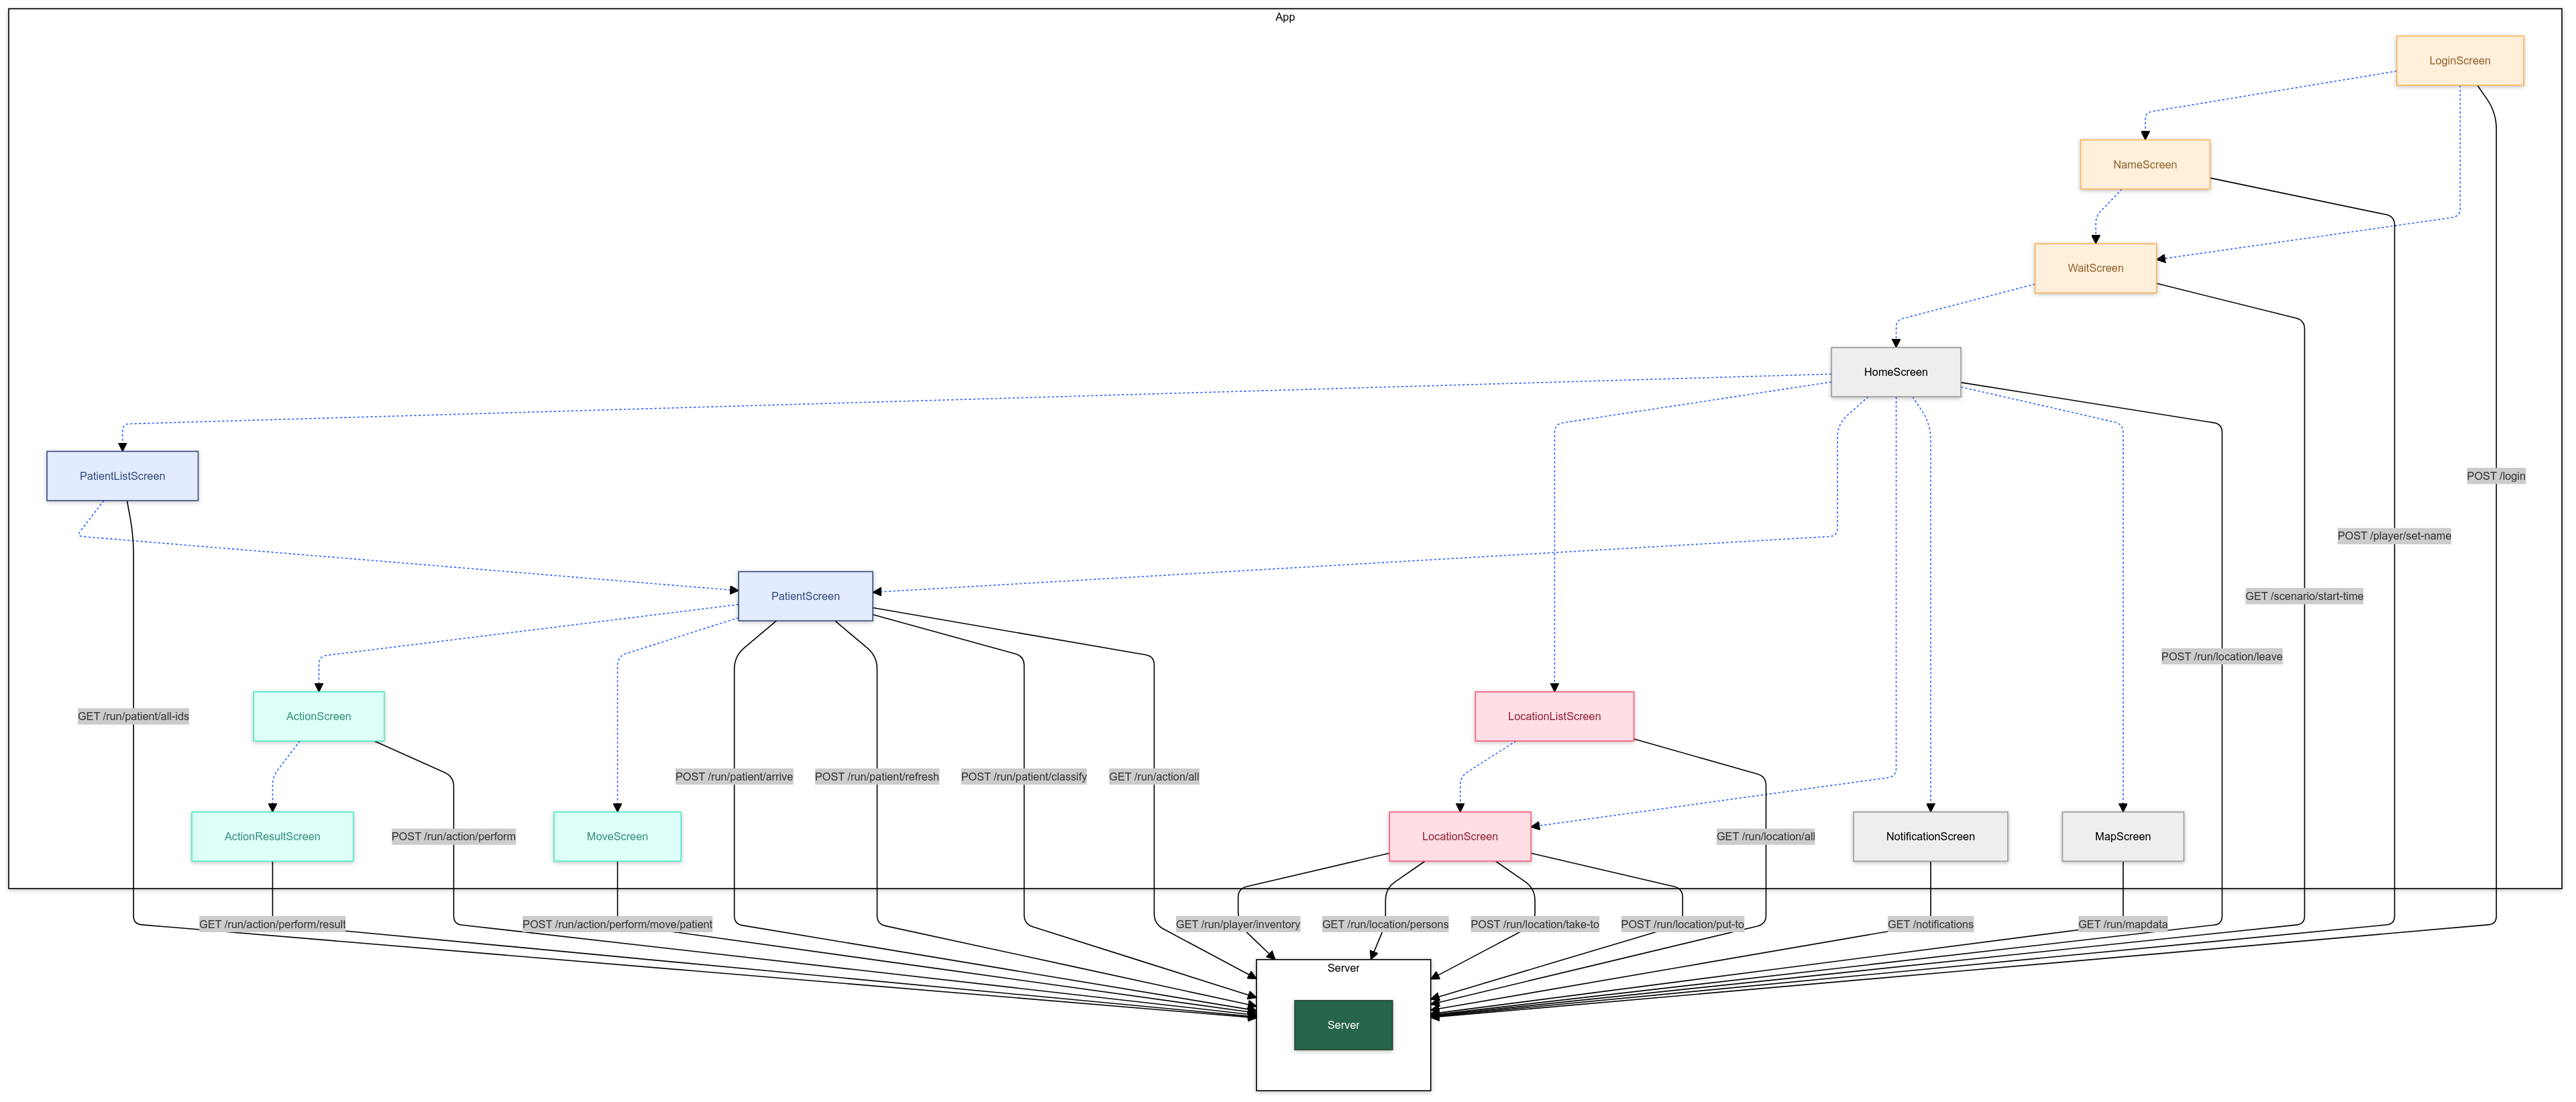
\includegraphics[width=1.0\textwidth]{images/app/server_endpoints.png}
\end{frame}

\begin{frame}{App - Kommunikation mit Server}
	\centering
	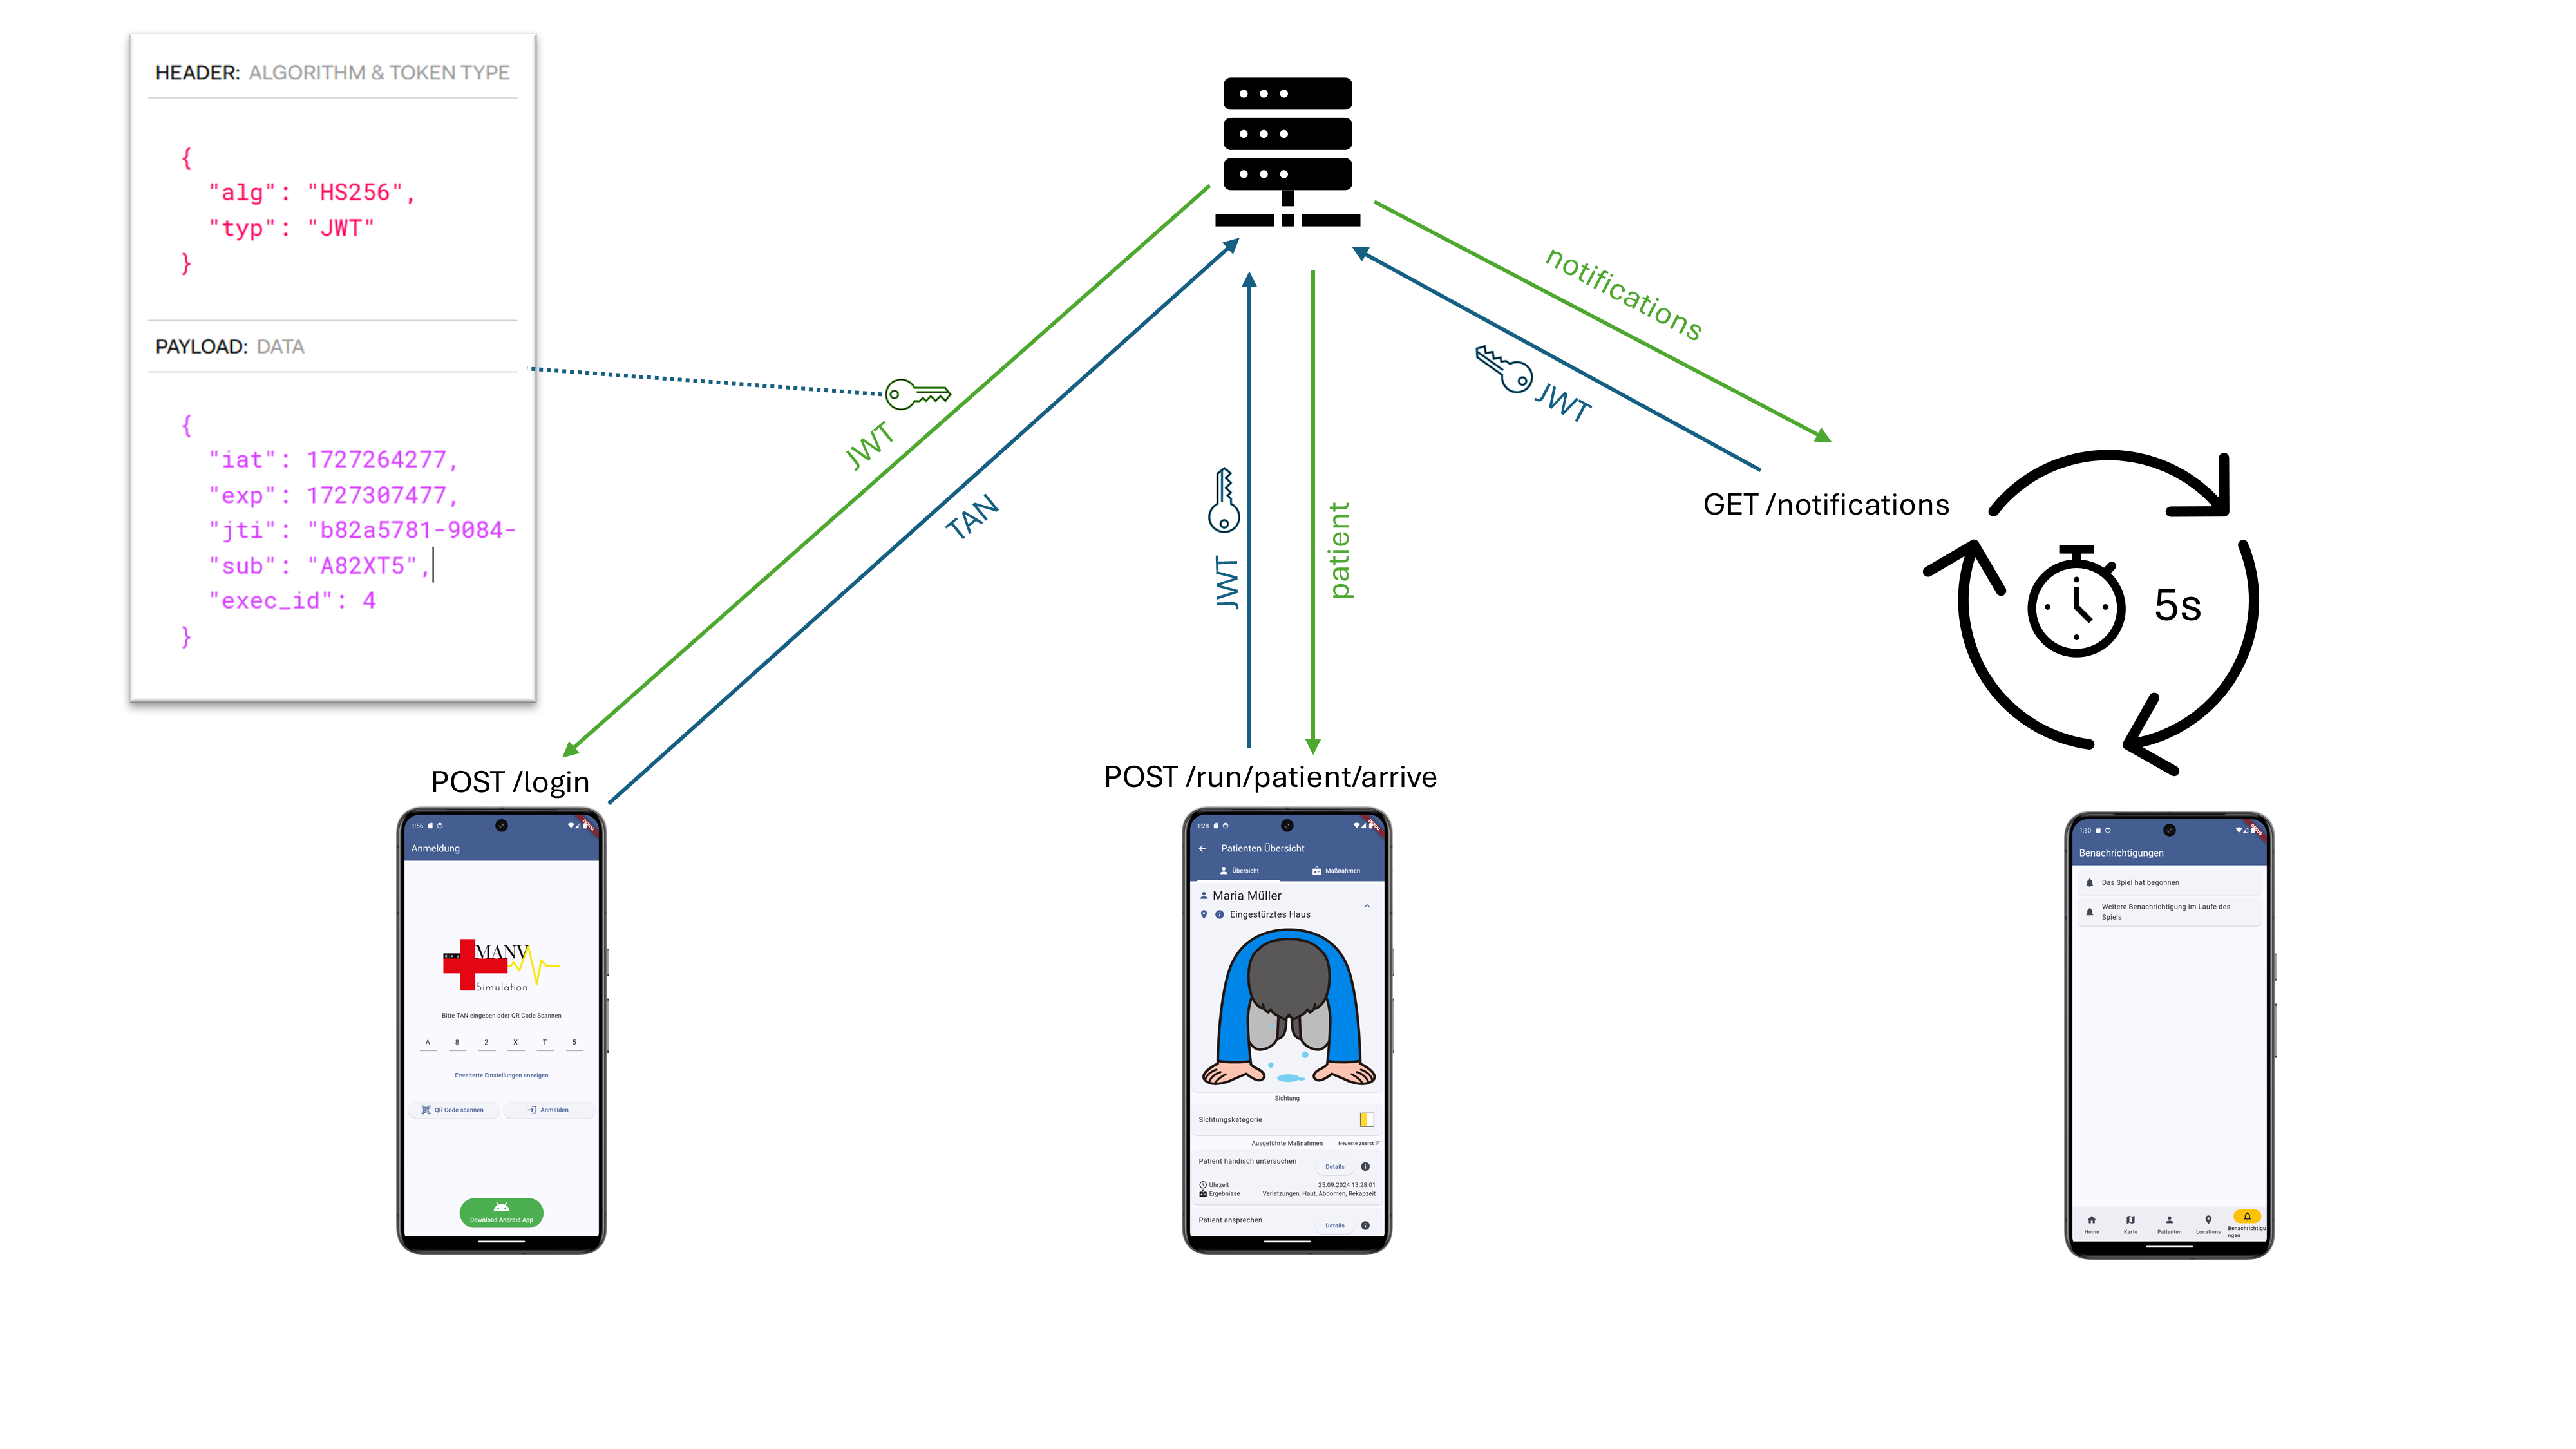
\includegraphics[width=1.0\textwidth]{images/app/api_flow.png}
\end{frame}

\begin{frame}{App - Kommunikation mit Server}
    \vfill
    \begin{figure}
        \centering
        \begin{minipage}{0.3\textwidth}
            \centering
            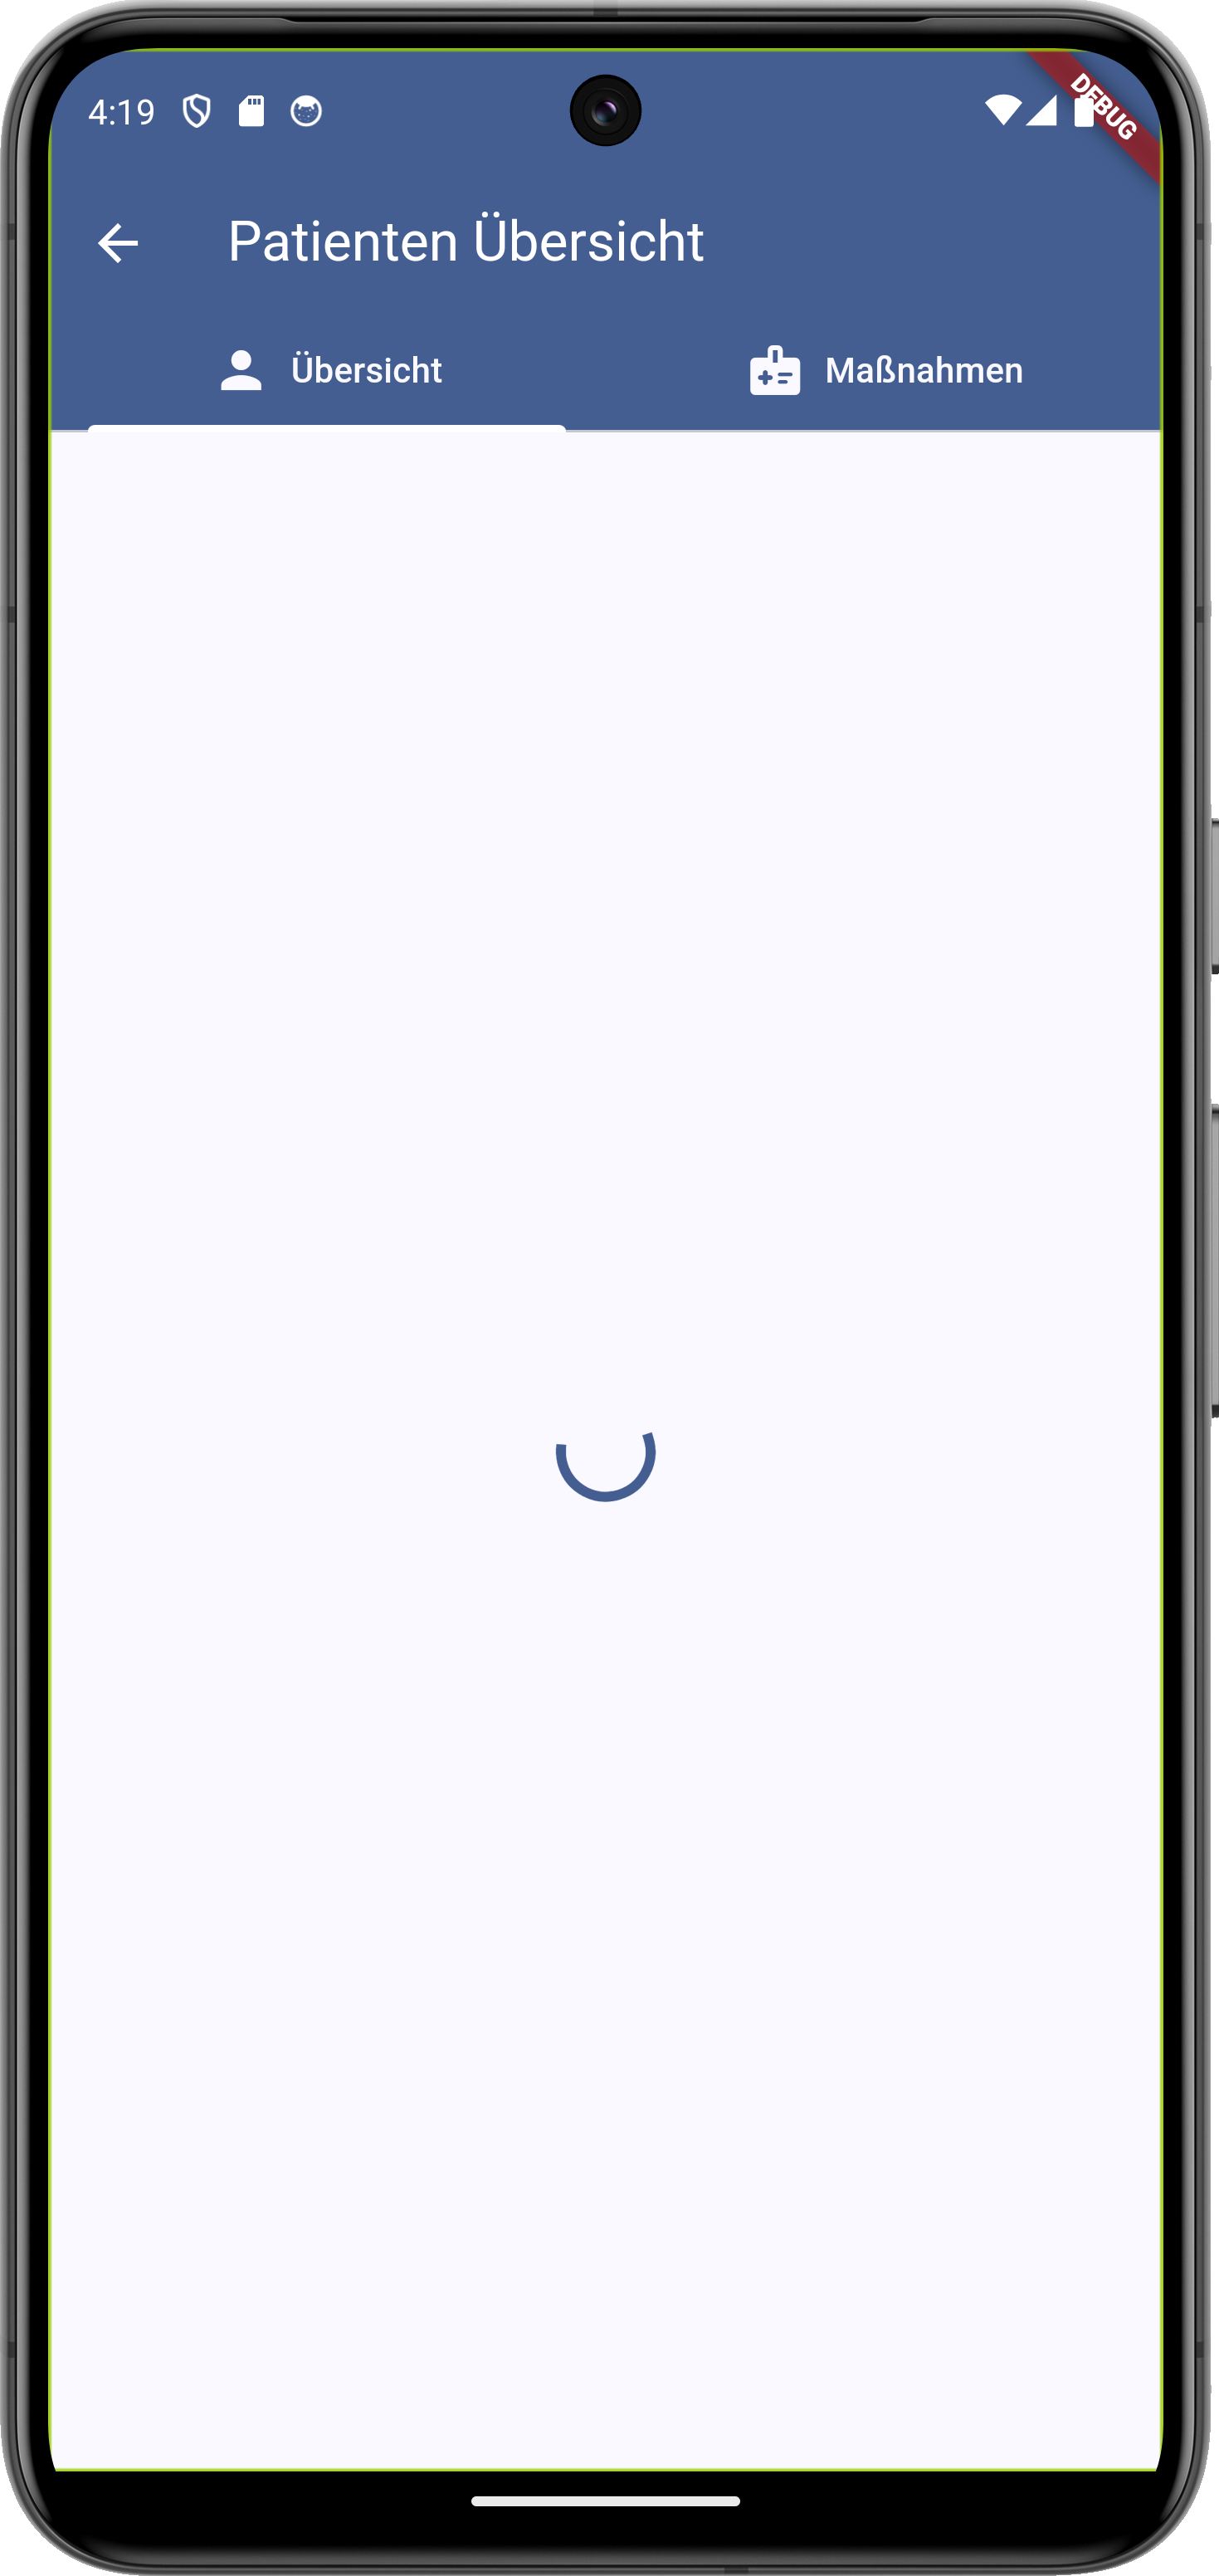
\includegraphics[height=0.8\textheight]{images/app/screenshots/concurrency_loading.png}
            \par{Laden}
        \end{minipage}
        \hspace{0.5cm}
        \begin{minipage}{0.3\textwidth}
            \centering
            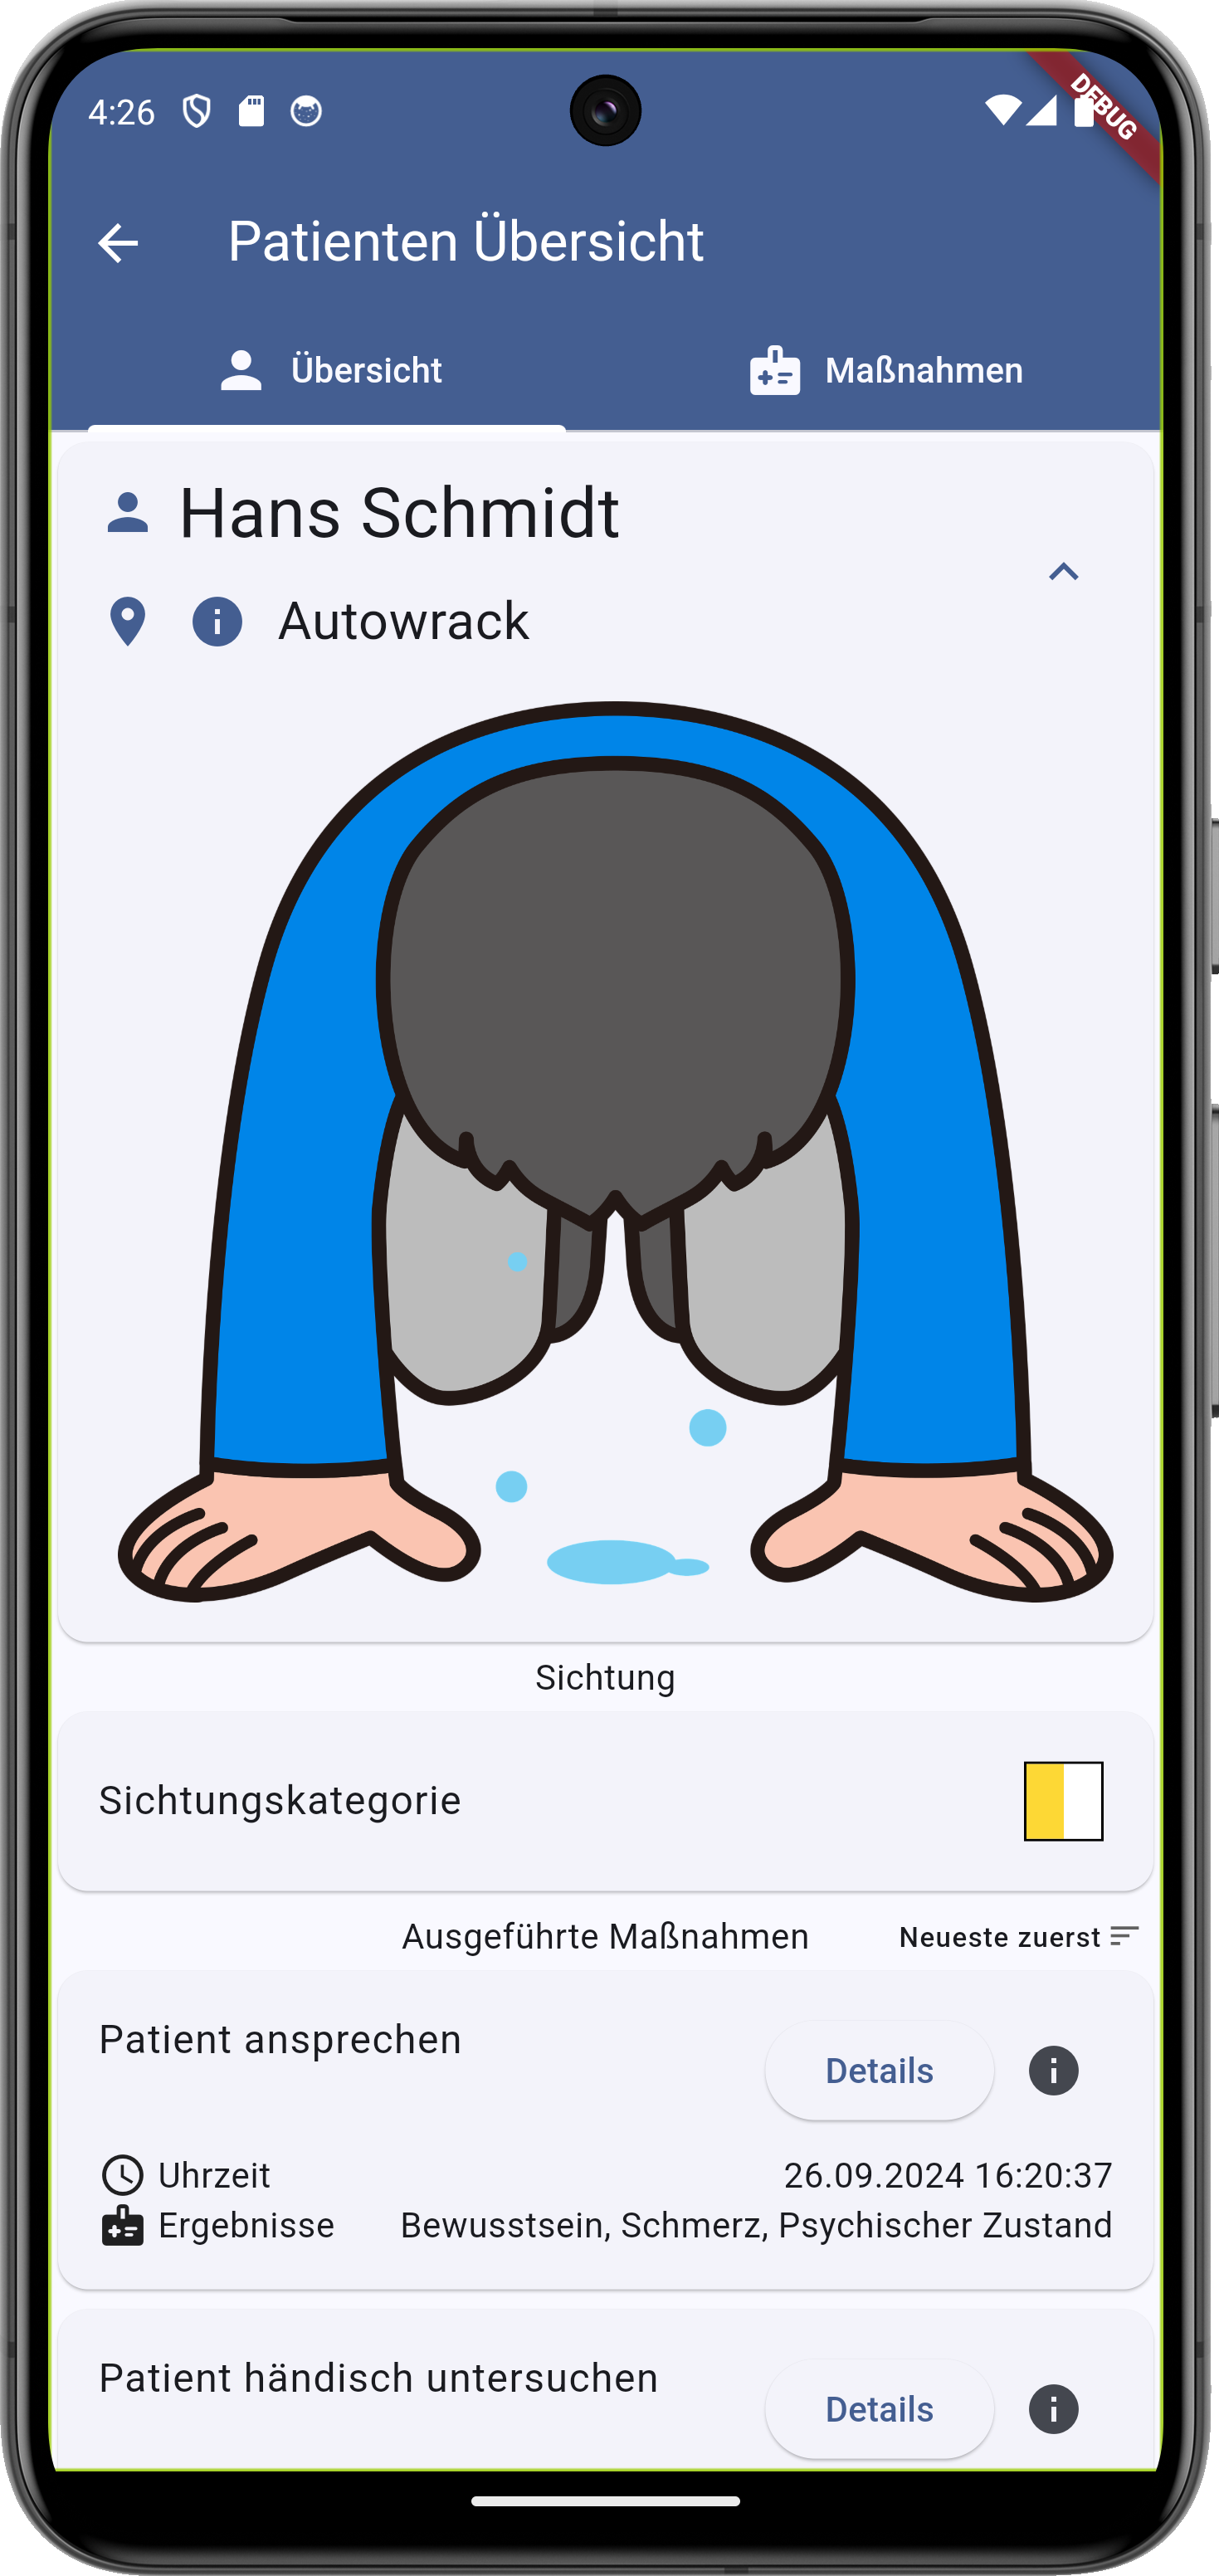
\includegraphics[height=0.8\textheight]{images/app/screenshots/concurrency_ok.png}
            \par{Ereignis}
        \end{minipage}
        \hspace{0.5cm}
        \begin{minipage}{0.3\textwidth}
            \centering
            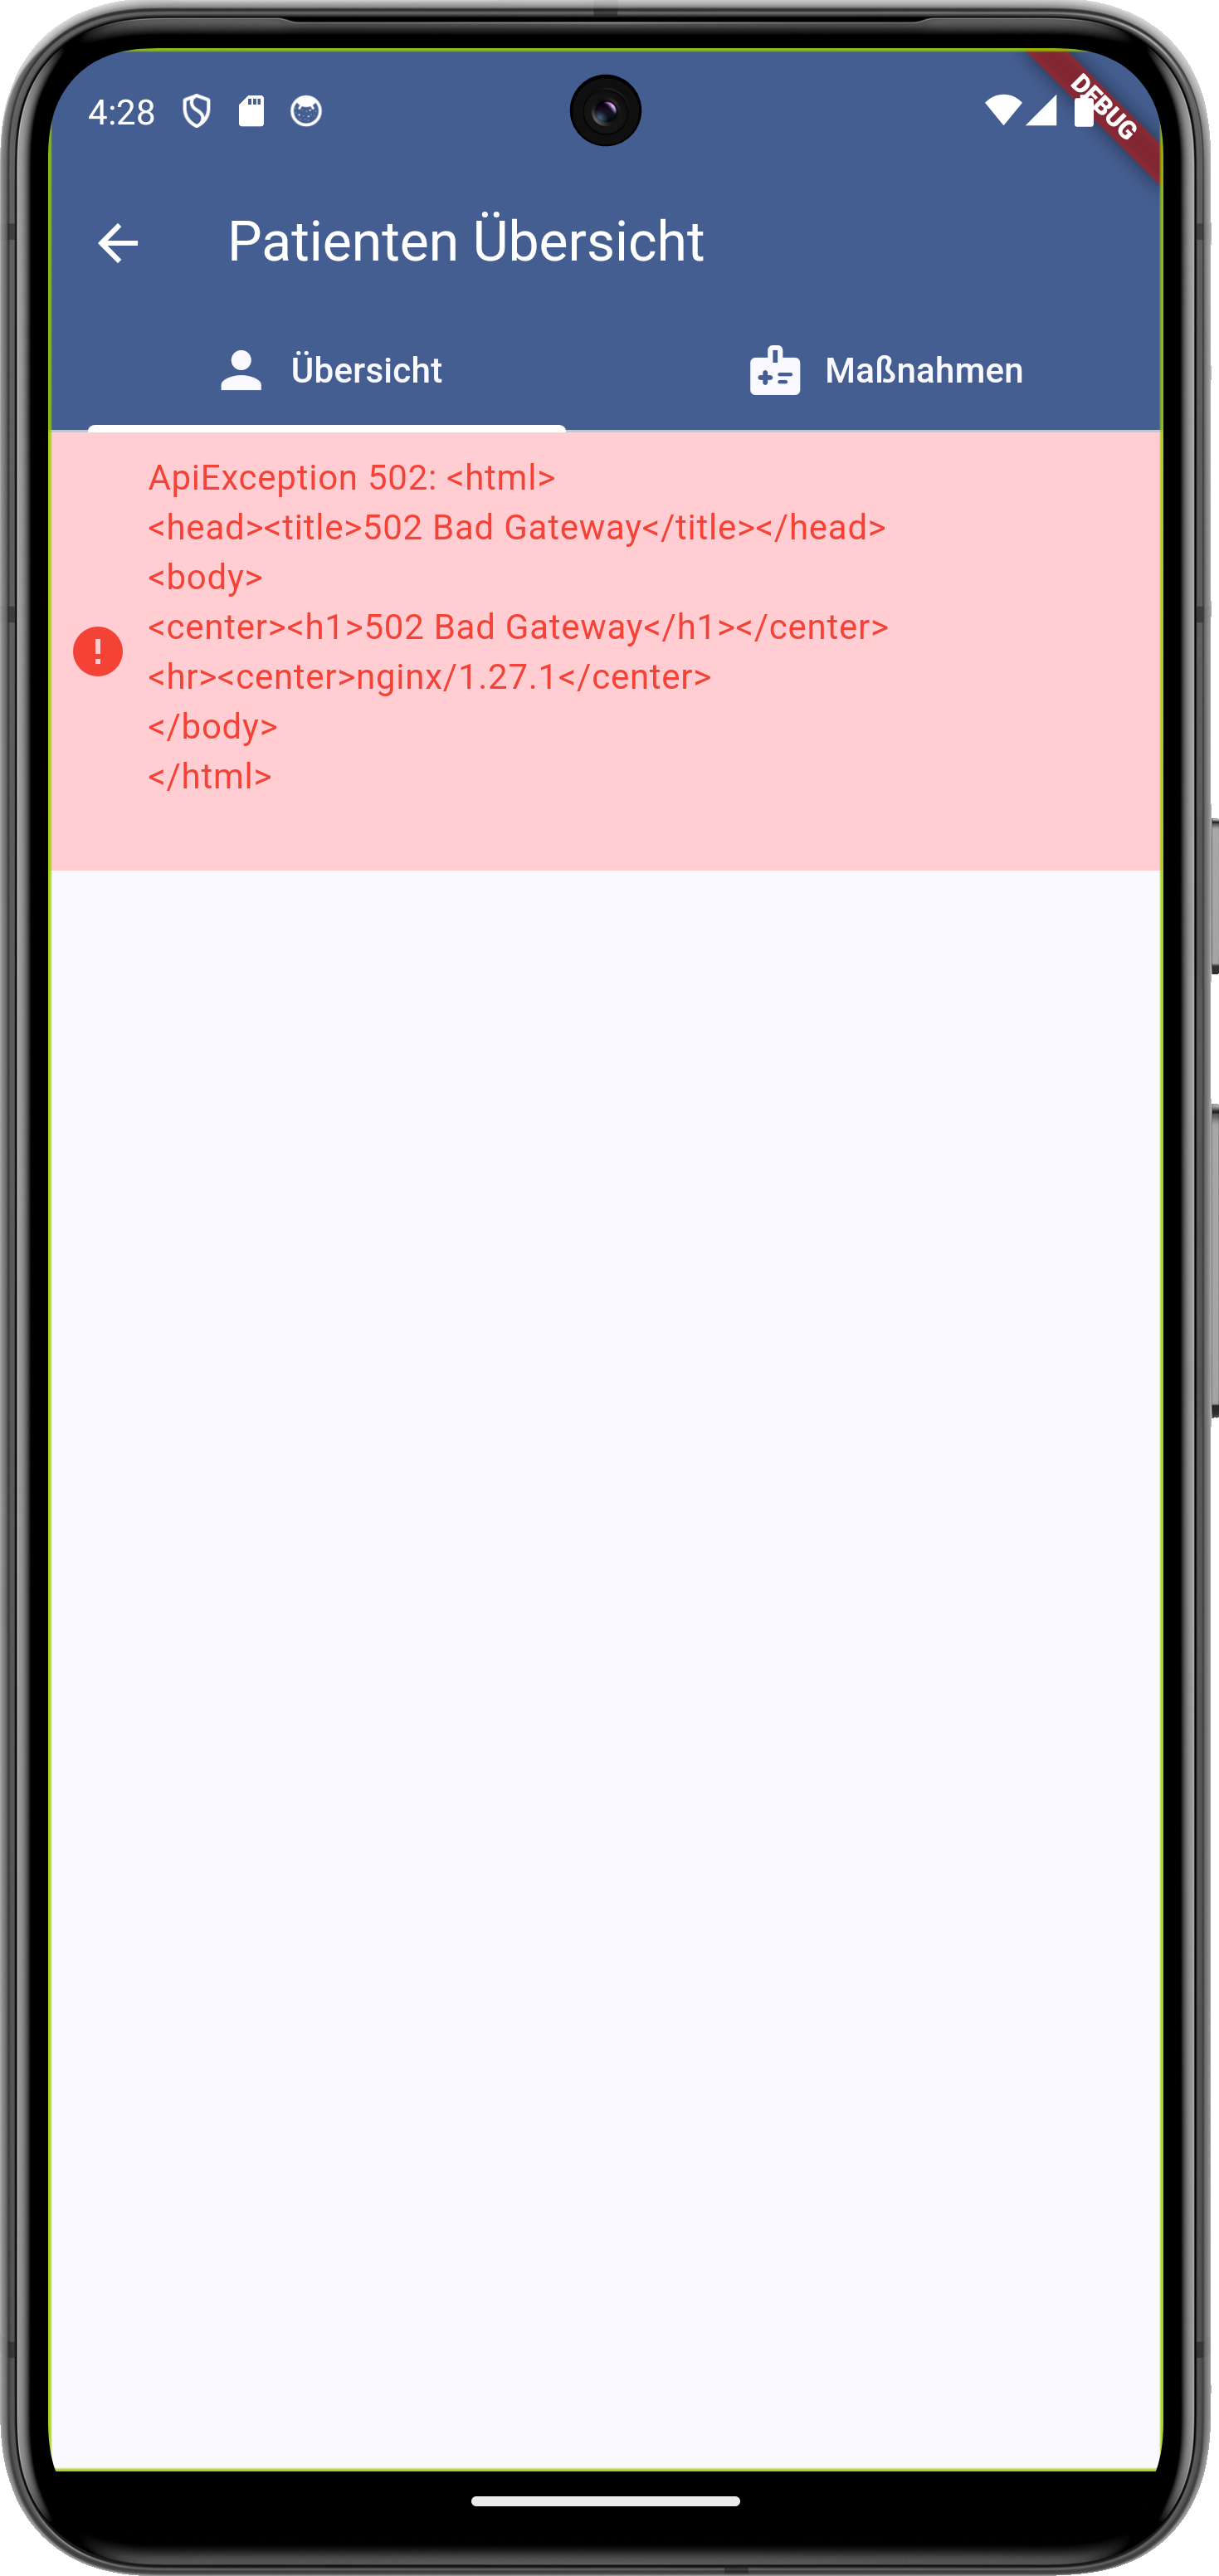
\includegraphics[height=0.8\textheight]{images/app/screenshots/concurrency_error.png}
            \par{Fehler}
        \end{minipage}
    \end{figure}
    \vfill
\end{frame}
